\section{Finite Element Models}
\label{FEMModels:sec}

This section details how to construct three-dimensional finite element models,
and how to couple them with the other simulation components described in
previous sections (e.g.~particles and rigid bodies).  Finite element
\emph{muscles}, which have additional properties that allow them to contract
given activation signals, are discussed in Section \ref{sec:fem:muscle}.

\subsection{Overview}
\label{sec:fem:overview}

The finite element method (FEM) is a numerical technique used for solving a 
system of partial differential equations (PDEs) over some domain.  The general
approach is to divide the domain into a set of building blocks, referred to
as \emph{elements}.  These partition the space, and form local domains over
which the system of equations can be locally approximated. The corners of these
elements, the \emph{nodes}, become control points in a discretized system.  
The solution is then assumed to be
smoothly interpolated across the elements based on values determined at the
nodes.  Using this discretization, the differential system is converted into 
an algebraic one, which is often linearized and iteratively solved.

In ArtiSynth, the PDEs considered are the governing equations of
continuum mechanics: the conservation of mass, momentum and energy.  To 
complete the system, a \emph{constitutive equation} is required that describes
the stress-strain response of the material.  This constitutive equation is what
disguishes between material types.  The domain is the three-dimensional space
that the model occupies. This must be divided into small elements which 
accurately represent the geometry. Within each element, the PDEs are
sampled at a set of points, referred to as \emph{integration points}, and 
terms are numerically integrated to form an algebraic system to solve.

The purpose of the rest of this section is to describe the construction and
use of finite elements models within ArtiSynth.  It does not further discuss 
the mathematical framework or theory.
For an in-depth coverage of the nonlinear finite element method, as applied
to continuum mechanics, the reader is referred to the textbook by Bonet and 
Wood \cite{bonet:fem:2000}.

\subsubsection{Component structure}
\label{sec:fem:structure}

The basic type of finite element model is implemented in the class 
\javaclass[artisynth.core.femmodels]{FemModel3d}.  This class controls some
properties that are used by the model as a whole.  The key ones that affect
simulation dynamics are:
\begin{center}
	\begin{tabular}{|ll|}
		\hline
		Property & Description\\
		\hline
		{\tt density} & The density of the model\\
		{\tt material} & An object that describes the material's 
		    \emph{constitutive law} (i.e.~its stress-strain relationship).\\
		{\tt particleDamping} & Proportional damping associated with the 
		    particle-like motion of the FEM nodes.\\
		{\tt stiffnessDamping} & Proportional damping associated with the 
		    system's stiffness term.\\
		\hline
	\end{tabular}
\end{center}
Keep in mind that ArtiSynth is essentially ``unitless'' (Section 
\ref{sec:mechii:units}), so it is the responsibility of the developer to
ensure that all properties are specified in a compatible way.  

The density of the model is used to compute the mass distribution throughout
the model.  Note that we use a \emph{diagonally lumped mass matrix} (DLMM)
formulation, so the mass is assumed to be concentrated at the location of
the discritized FEM nodes.  To allow for a spatially-varying density,
a mass can later be specified for each node individually.

The FEM's {\tt material} is a delegate object used to compute stress and 
stiffness within individual elements.  It handles the \emph{constitutive}
component of the model.  Materials will be discussed in more detail in
Section \ref{sec:fem:materials}.

\paragraph{Damping}

ArtiSynth uses \emph{Rayleigh damping} to dissipate energy within finite
element models.  This is composed of a combination of two proportional
damping terms: one related to the system's mass, and one related to
stiffness.

The ``particle damping'' (otherwise known as ``mass damping'') property 
of the \javaclass[artisynth.core.femmodels]{FemModel3d} class
specifies the damping coefficient associated with the model's mass.  This 
induces a force acting against motion of FEM nodes:
\begin{align}
\f_M & = -d_M \M\v, \label{eqn:massdamping} 
\end{align}
where $d_M$ is the value of {\tt particleDamping}, $\M$ is the FEM model's
lumped mass matrix, and $\v$ is the vector of concatenated node velocities.
Since $\M$ is diagonal, this expression is essentially the same as the
``point damping'' described in Equation \eqref{eq:pointdamping}.  To complete
Rayleigh damping, a ``stiffness damping'' term is added:
\begin{align}
\f_K & = -d_K\K\v, \label{eqn:stiffnessdamping}
\end{align}
where $d_K$ is the value of {\tt stiffnessDamping}, and $\K$ is the FEM's
stiffness matrix.

\paragraph{Sub-components}

Each FEM model contains at least three lists of sub-components:

\begin{description}
\item[Nodes]\mbox{}

The particle-like dynamic components of the model.  These lie at the corners
of the elements, and carry all the mass.

\item[Elements]\mbox{}

The spatial building blocks of the model.  These define the sub-units over 
which the system is numerically integrated.

\item[Meshes]\mbox{}

The geometry in the model.  This will include the surface mesh, and any other
embedded geometries which are used for either display purposes, or for physical
interactions (e.g.~collision).
\end{description}


\subsubsection{Materials}
\label{sec:fem:materials}

\subsubsection{Boundary conditions}

\subsection{FEM model creation}

\subsubsection{Using factory methods}

\subsubsection{Using external meshes}

\subsubsection{Using direct code}

\subsubsection{A simple beam model}

\begin{figure}[ht]
\begin{center}
\iflatexml
 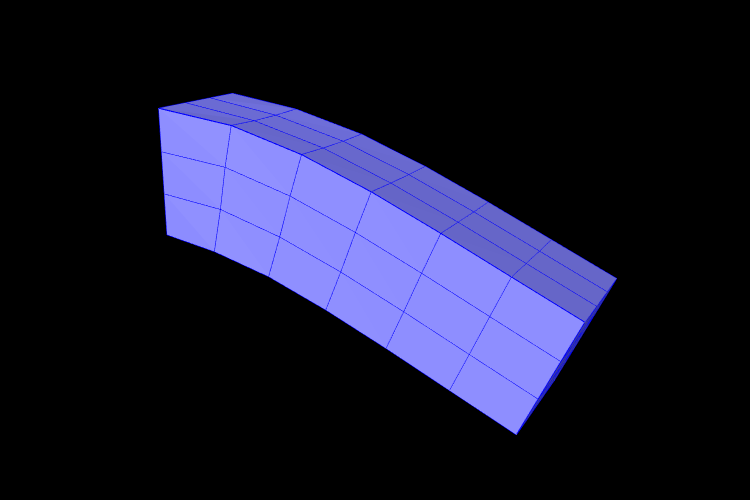
\includegraphics[]{images/FemBeam}
\else
 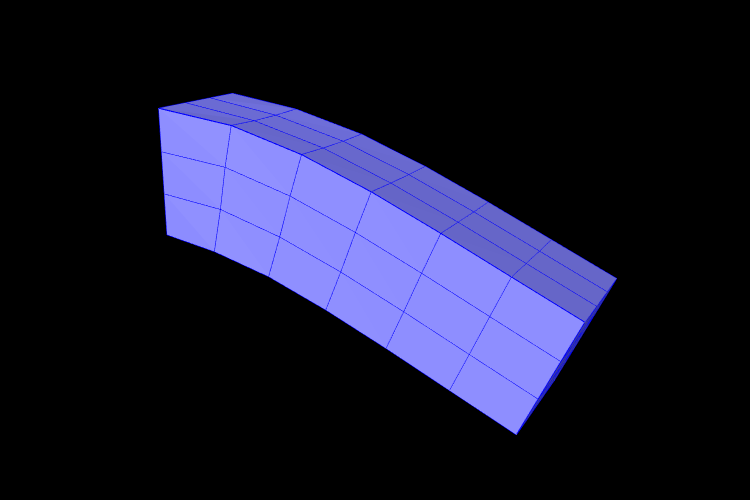
\includegraphics[width=3.75in]{images/FemBeam}
\fi
\end{center}
\caption{FemBeam model loaded into ArtiSynth.}
\label{FemBeam:fig}
\end{figure}

\subsection{FEM Geometry}

\subsubsection{Surface meshes}

\subsubsection{Embedding geometry within an FEM}

\subsubsection{A beam with an embedded sphere}

% EmbeddedFemSphere

\subsection{Node attachments}
\label{NodeAttachments:sec}

\subsubsection{General principles}

\subsubsection{Connecting a beam to a block}

\begin{figure}[ht]
\begin{center}
\iflatexml
 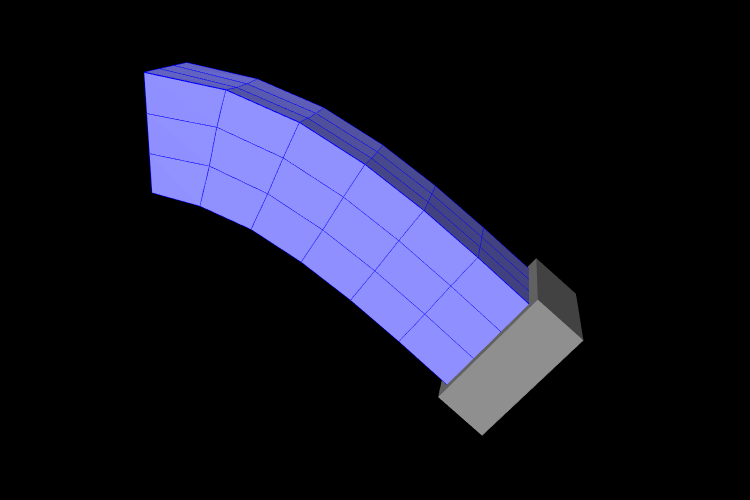
\includegraphics[]{images/FemBeamWithBlock}
\else
 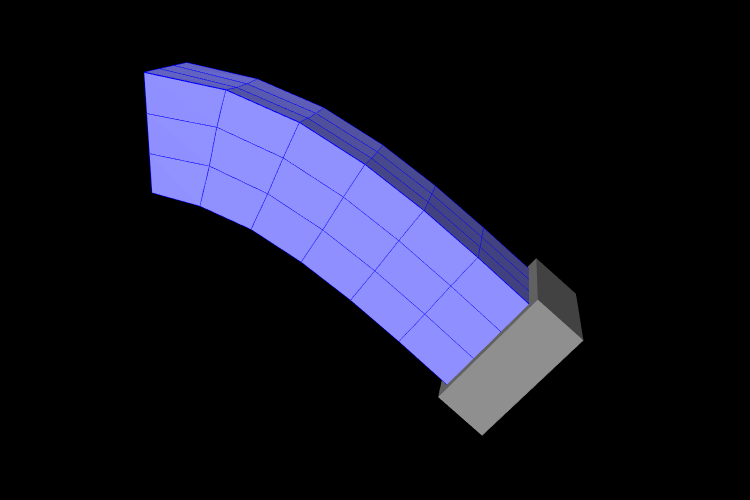
\includegraphics[width=3.75in]{images/FemBeamWithBlock}
\fi
\end{center}
\caption{FemBeamWithBlock model loaded into ArtiSynth.}
\label{FemBeamWithBlock:fig}
\end{figure}

% FemBeamWithBlock

\subsubsection{Connecting two FEMs together}

% ConnectedFems

\subsection{FEM markers}

\subsubsection{Embedding particles in FEMs}

\subsubsection{Attaching a FEM beam to a muscle}

\begin{figure}[ht]
\begin{center}
\iflatexml
 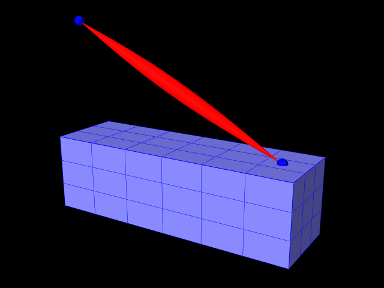
\includegraphics[]{images/FemBeamWithMuscle}
\else
 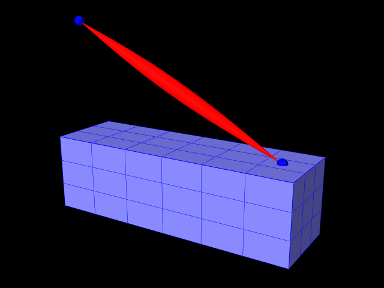
\includegraphics[width=3.75in]{images/FemBeamWithMuscle}
\fi
\end{center}
\caption{FemBeamWithMuscle model loaded into ArtiSynth.}
\label{FemBeamWithMuscle:fig}
\end{figure}

% FemBeamWithMuscle

\subsection{Muscle activated FEM models}
\label{sec:fem:muscle}

\subsubsection{FemMuscleModel}

\subsubsection{Activation with fibres}

\subsubsection{Activation with embedded materials}

\subsubsection{Comparision with two beam examples}

\begin{figure}[ht]
\begin{center}
\iflatexml
 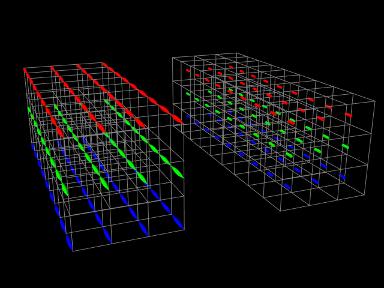
\includegraphics[]{images/FemMuscleBeams}
\else
 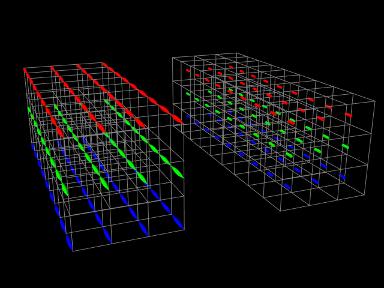
\includegraphics[width=3.75in]{images/FemMuscleBeams}
\fi
\end{center}
\caption{FemMuscleBeams model loaded into ArtiSynth.}
\label{FemMuscleBeams:fig}
\end{figure}

% FemMuscleBeams

\subsection{Collisions}

\subsubsection{Colliding with FEM geometry}

\subsubsection{Colliding with the surface mesh}

\begin{figure}[ht]
\begin{center}
\iflatexml
 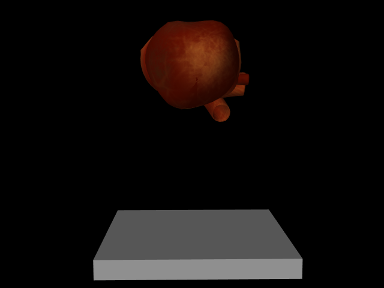
\includegraphics[]{images/FemMuscleHeart}
\else
 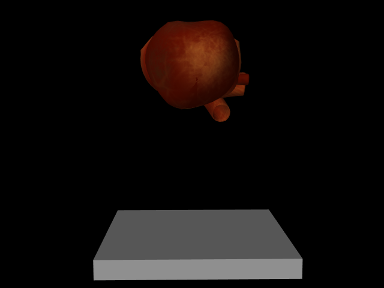
\includegraphics[width=3.75in]{images/FemMuscleHeart}
\fi
\end{center}
\caption{FemMuscleHeart model loaded into ArtiSynth.}
\label{FemMuscleHeart:fig}
\end{figure}

% FemMuscleHeart

\subsubsection{Colliding with an embedded sphere}

\begin{figure}[ht]
\begin{center}
\iflatexml
 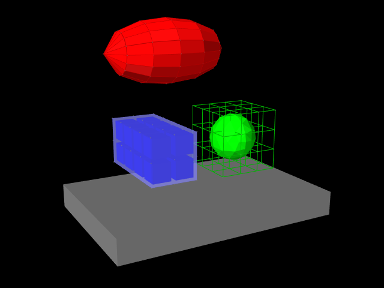
\includegraphics[]{images/FemCollisions}
\else
 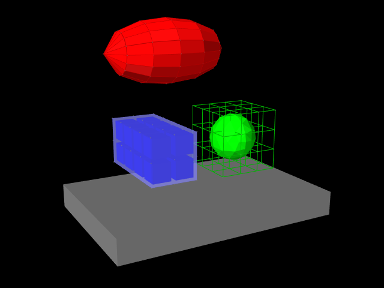
\includegraphics[width=3.75in]{images/FemCollisions}
\fi
\end{center}
\caption{FemCollisions model loaded into ArtiSynth.}
\label{FemCollisions:fig}
\end{figure}

\subsection{Visualization}

stuff stuff stuff

\subsubsection{Rendering settings}

stuff stuff stuff

\subsubsection{Stress and strain plotting}

stuff stuff stuff
